% Evidence-backed draft, aligned with the agentic prototype on 2026-09-09.
% Reported results cover 60 controlled runs over 15 registered questions plus
% two registered CoDA-Bench questions in a second community; do not remove the
% deterministic/non-held-out scope qualification. Live-model smoke observations
% are recorded separately in docs/agentic-smoke-evidence.md and
% docs/stage-io-validation.md, not pooled as accuracy.
% Keep the two marked VLDB blocks unchanged.

\documentclass[sigconf, nonacm]{acmart}

%%% do not modify the following VLDB block %%
%%% VLDB block start %%%
\usepackage{pvldb}
%%% VLDB block end %%%

\renewcommand\vldbdoi{XX.XX/XXX.XX}
\renewcommand\vldbpages{XXX-XXX}
\renewcommand\vldbavailabilityurl{}

\newcommand{\systemname}{\textsc{Ask, Don't Upload}}
\setlength{\emergencystretch}{1em}
\setlength{\vfuzz}{2pt}

\begin{document}

\title{Ask, Don't Upload: A Question-Driven Agentic System for Closed-Loop
Data Discovery, Preparation, and Analysis}

% TODO(author): The VLDB 2027 Demo CFP was not linked on the official site as of 2026-09-09;
% do not infer its anonymity rule from the Research Track. Replace this block
% only after the Demo CFP appears and every author confirms the metadata.
\author{Author Name}
\affiliation{%
  \institution{Institution}
  \city{City}
  \country{Country}
}
\email{author@example.com}

\begin{abstract}
Source relevance is not analytical sufficiency: a plausible table can prove
inadequate when a downstream join or statistical operation executes.  We
present \systemname, a question-driven system that makes data discovery a
revisable part of analytical execution.  For each question, an Analytical
Sufficiency Contract (ASC) turns coverage, join, statistical, and claim-lineage
requirements into executable obligations.  When execution exposes an unmet
obligation, a typed repair goal can reopen Discovery and trigger downstream
rematerialization before report release.  The Web demo exposes community
navigation, preparation schemas and candidates, and analysis-to-report execution
across 30 open CoDA-Bench communities using one external model.
An offline registry isolates the repair mechanism.  Across
all 15 questions assigned to one CoDA-Bench community---ten direct, four
cross-source, and one with an unavailable referenced source---closed-loop
execution produces 14 exact reports and the correct local data-gap diagnosis.
Linear execution resolves 11/15 terminal outcomes.  A same-budget static retry
that ignores violation-specific search terms resolves 13/15 with 21 source
profiles and seven repairs; typed repair resolves 15/15 with 18 profiles and
four repairs.  Full profiling also resolves 15/15 but logically requests 150
profiles.  Two registered tasks in a second community match exactly.  These
deterministic, task-registered results establish mechanism feasibility, not
open-ended generality.
\end{abstract}

\maketitle

%%% do not modify the following VLDB block %%
%%% VLDB block start %%%
\vldbtopmatter
%%% VLDB block end %%%

\section{Introduction}

Consider 2016 Grade-8 SHSAT participation and school demographics.  A registration
table contains year, grade, school identifier, and test counts, but not
demographics.  Valid preparation code cannot supply the missing evidence;
the source decision must be revisited downstream.

Recent demonstrations cover much of the question-to-result path. TableCopilot
and Sentence to Model connect natural-language requests to table discovery or
data collection~\cite{cui2025tablecopilot,einy2025sentence}. QueryArtisan,
Graphy, DA-Studio, and DeepEye expose end-to-end analysis, reporting, or
steering~\cite{liu2025queryartisan,lai2025graphy,liu2026dastudio,li2026deepeye}.
Carnot and Credo expose inspectable or adaptive execution
~\cite{russo2026carnot,lu2026credo}; Trace Integrity studies trace-to-answer
linkage~\cite{dutta2026trace}. Our control point is for downstream evidence to invalidate and
repair an upstream source decision, then replay preparation and analysis, under
a question-only contract.

\systemname{} addresses this gap over a pre-authorized noisy data
environment.  The user supplies only an analytical question for each task---no
filename, schema, join path, preparation plan, or report outline.  The system
returns either an evidence-grounded report or a typed insufficiency diagnosis.
It builds on CoDA-Bench~\cite{zhang2026codabench} for a noisy, data-intensive
task setting; DeepPrep~\cite{fan2026deepprep} for execution-grounded
materialization and non-local revision; and DeepAnalyze~
\cite{zhang2025deepanalyze} for the analysis-to-report scope.  Its distinct
runtime mechanism, illustrated in Figure~\ref{fig:overview}, extends revision
across the entire data lifecycle.

We make three concrete contributions:

\begin{itemize}
  \item \textbf{Contract:} an executable ASC that turns measure, dimension,
  coverage, grain, join, statistical, and evidence failures into repair targets;
  \item \textbf{Closed loop:} a materialized lifecycle graph where typed
  violations create targeted backward edges to Discovery followed by downstream
  rematerialization; and
  \item \textbf{Demo and evidence:} a deployable question-only interface
  exposing stage inputs/outputs, repair, abstention, and claim lineage,
  backed by a complete 15-task community census.
\end{itemize}

\section{System Overview}

\begin{figure*}[t]
  \centering
  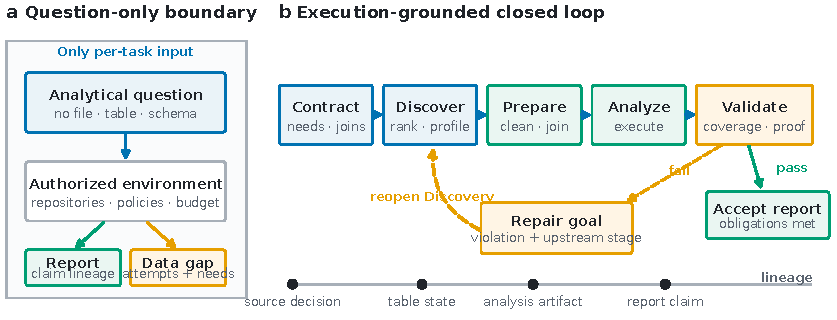
\includegraphics[width=\textwidth]{figures/system-overview.pdf}
  \caption{The question-only boundary (a) and closed-loop runtime (b).
  Solid arrows are forward execution; the dashed orange path is a typed
  downstream violation that reopens an upstream decision.  Stable identifiers
  connect source decisions, materialized tables, analysis artifacts, and report
  claims.}
  \Description{A two-panel architecture diagram. The left panel shows an
  analytical question as the only per-task input to an authorized environment,
  which returns a report or typed gap. The right panel shows Contract, Discover,
  Prepare, Analyze, and Validate stages, with a dashed repair arrow returning
  from a failed validation to Discovery and a lineage chain below.}
  \label{fig:overview}
\end{figure*}

\subsection{Question-Only Contract}

At deployment time, an administrator defines an environment
$E=(D,P,B)$ comprising data repositories $D$, access policies $P$, and an
execution budget $B$.  A task supplies only a natural-language question $q$.
The compiler produces

\[
  \mathrm{ASC}(q)=\langle O_m,O_d,O_c,O_g,O_j,O_s,O_e\rangle,
\]

where obligations cover measures, dimensions, entity/time coverage, grain,
joins, statistical preconditions, and claim evidence.  Each stores an expected
condition, an executable check, status, and evidence references.  For SHSAT,
checks include demographic coverage, sufficient complete pairs, and join
coverage.  The ASC is an operational contract, not a completeness proof.

\subsection{Materialized Closed-Loop Execution}

The controller maintains typed source decisions, table states, analysis
artifacts, claims, and events with stable IDs.  Discovery profiles chosen
assets, recording paths, schemas, sizes, row counts, and content hashes.
Preparation materializes a state with parent/source IDs; Analysis consumes it
and emits artifacts or a \emph{sufficiency violation}.

A violation identifies the failed obligation, observed and expected values,
the detection stage, the responsible upstream stage, and supporting evidence.
The controller compiles it into a repair goal.  Missing analytical columns, for
example, target Discovery with the absent dimensions as new search terms.  A
subsequent source decision records the triggering violation; affected
preparation and analysis are replayed from the prior materialized state.  A
report is released only after all required obligations pass and every numeric
claim references an analysis artifact and executable evidence.  Otherwise
the run stops with a data gap, exhausted budget, or unsupported capability.
Unimplemented operators and Discovery turn exhaustion are not data gaps;
a model-reported gap is a bounded search judgment, not an exhaustive catalog
certificate.

\subsection{Agents and Stage Outputs}

One external model drives discovery, candidate planning, repair, and report
synthesis; no supporting paper's trained model is loaded.
The pinned CoDA-Bench open pool contains 30 communities, 196 source datasets,
and 30,292 discoverable files, including 16,315 CSVs.  One evaluation community
remains excluded.  Discovery searches paths and traverses directories, obtaining
schemas and bounded previews by inspection before selecting files within one
community.  Global routing extends CoDA-Bench's given-community task setting;
file counts measure catalog coverage, not solved tasks.

Preparation adapts DeepPrep's tree-based reasoning to declarative candidates.
Each expansion submits a complete operator plan and may name any earlier
successful candidate as its parent.  Schema validation precedes execution,
which produces immutable tables, operator observations, and sufficiency checks.
The tree separates rejected proposals from executed states; termination selects
a successful candidate.  Input/output schemas and five-row previews expose
the transformation.

Analysis adapts DeepAnalyze's execution-feedback interface.  The local compiler
executes visible SQL or restricted Python and checks results against the
dataframe engine; failures create Debug cells and dataframe fallbacks.  These
are compiled cells, not arbitrary model-authored programs.  A final model call
organizes executed artifacts into an executive summary, evidence-linked
sections, conclusion, and limitations.  Unknown references, omitted artifacts,
or malformed drafts trigger bounded correction or a deterministic fallback.
Reference integrity does not establish semantic entailment.  Broad recommendations
must expose missing dimensions and weights rather than invent a universal score.

\begin{table*}[t]
  \caption{Agentic demonstration path. Each visible step
  corresponds to persisted execution state rather than a scripted animation.}
  \label{tab:script}
  \small
  \begin{tabular}{p{0.11\textwidth}p{0.22\textwidth}p{0.28\textwidth}p{0.30\textwidth}}
    \toprule
    Stage & Attendee action & Immediate response & Technical point exposed \\
    \midrule
    1. Ask & Enter an analytical question; attach no data. &
      The run begins in the 30-community authorized pool. &
      A question is the only task-level input. \\
    2. Discover & Select a recorded hop. &
      The left inspector explains its action; the right community graph
      emphasizes the current edge over earlier paths. &
      Progressive community routing and inspected CSV selection. \\
    3. Prepare & Inspect a candidate and its table output. &
      Input schemas, operators, rejected/selected branches, and the prepared
      schema and rows appear together. &
      Execution-observed preparation with revisable candidates. \\
    4. Analyze & Open a code cell or a report section. &
      Executed SQL/Python, observations, charts, and a multi-section conclusion
      share artifact references. &
      A visible route from prepared data to report evidence. \\
    5. Revisit & Inspect a repair or run the offline gap example. &
      A typed violation reopens Discovery, or the run stops with an explicit gap. &
      Cross-stage revision and evidence-aware stopping. \\
    \bottomrule
  \end{tabular}
\end{table*}

\subsection{Deployment and Evaluation Modes}

Nginx connects React to FastAPI; browser polling reads persisted progress.
Docker mounts sources read-only, separately from runtime tables and reports.
The provider receives bounded metadata, previews, and observations:
``Don't Upload'' excludes user uploads, not server-to-model exchange.

A separate offline registry covers 17 inspected benchmark questions with
trusted operators and per-CSV SHA-256 checks.  It supplies the controlled
results and provider-independent fallback, not language-generalization
evidence.  Audience inspection supplies no sources, joins, or repair instructions.

\section{Demonstration Experience}

Three full-width stage tabs expose inputs and outputs.  The membership graph
shows all communities and only files encountered up to the selected hop;
arrows mark tool-focus transitions, not semantic similarity.  Completed runs
foreground the report, with source metadata, ASC, repair, and lineage available
on demand. Table~\ref{tab:script} specifies interaction, not fixed model latency.
Four registered offline examples provide a reproducible fallback.

\subsection{Contrasting Live Scenarios}

In the controlled task-959 repair, Discovery first selects a 140-row
SHSAT registration table.  After filtering to Grade 8 and 2016, Analysis finds
that Asian, Black/Hispanic, and White percentages are absent.  The visible
\texttt{analysis $\rightarrow$ discovery} repair adds a 1,272-row School
Explorer table, normalizes percentages, and joins \texttt{DBN} to
\texttt{Location Code}.  All 21 left-side records match.  The final report gives
correlations $0.434725$, $-0.513048$, and $0.586734$, with one executed artifact
reference per claim.

Task 960 repairs incomplete restaurant coverage by adding another nutrition
source.  Task 176 completes directly, showing that repair is conditional.
Task 179 references an attendance source absent from the pinned archive;
exhaustive inspection yields \texttt{data\_gap}.  Tasks 175 and 955 provide
two further missing-column repairs.  Benchmark answers are confined to the
post-run evaluator.

Figure~\ref{fig:interface} replays a recorded model smoke asking only, in Chinese, ``Which country is most
suitable for immigration?''  With neither user-supplied dimensions nor weights,
12 discovery records, including the root, lead to an 80-row 2020 quality-of-life
table.  One successful preparation candidate and ten analysis artifacts yield
a five-section report separating the dataset's overall ranking from individual
dimensions and missing policy evidence.  This post-fix demonstration followed
cross-community selection and operator-schema defects; it is neither a
first-pass success-rate estimate, evidence of non-local backtracking, nor a
validation of actual immigration suitability.

\begin{figure*}[t]
  \centering
  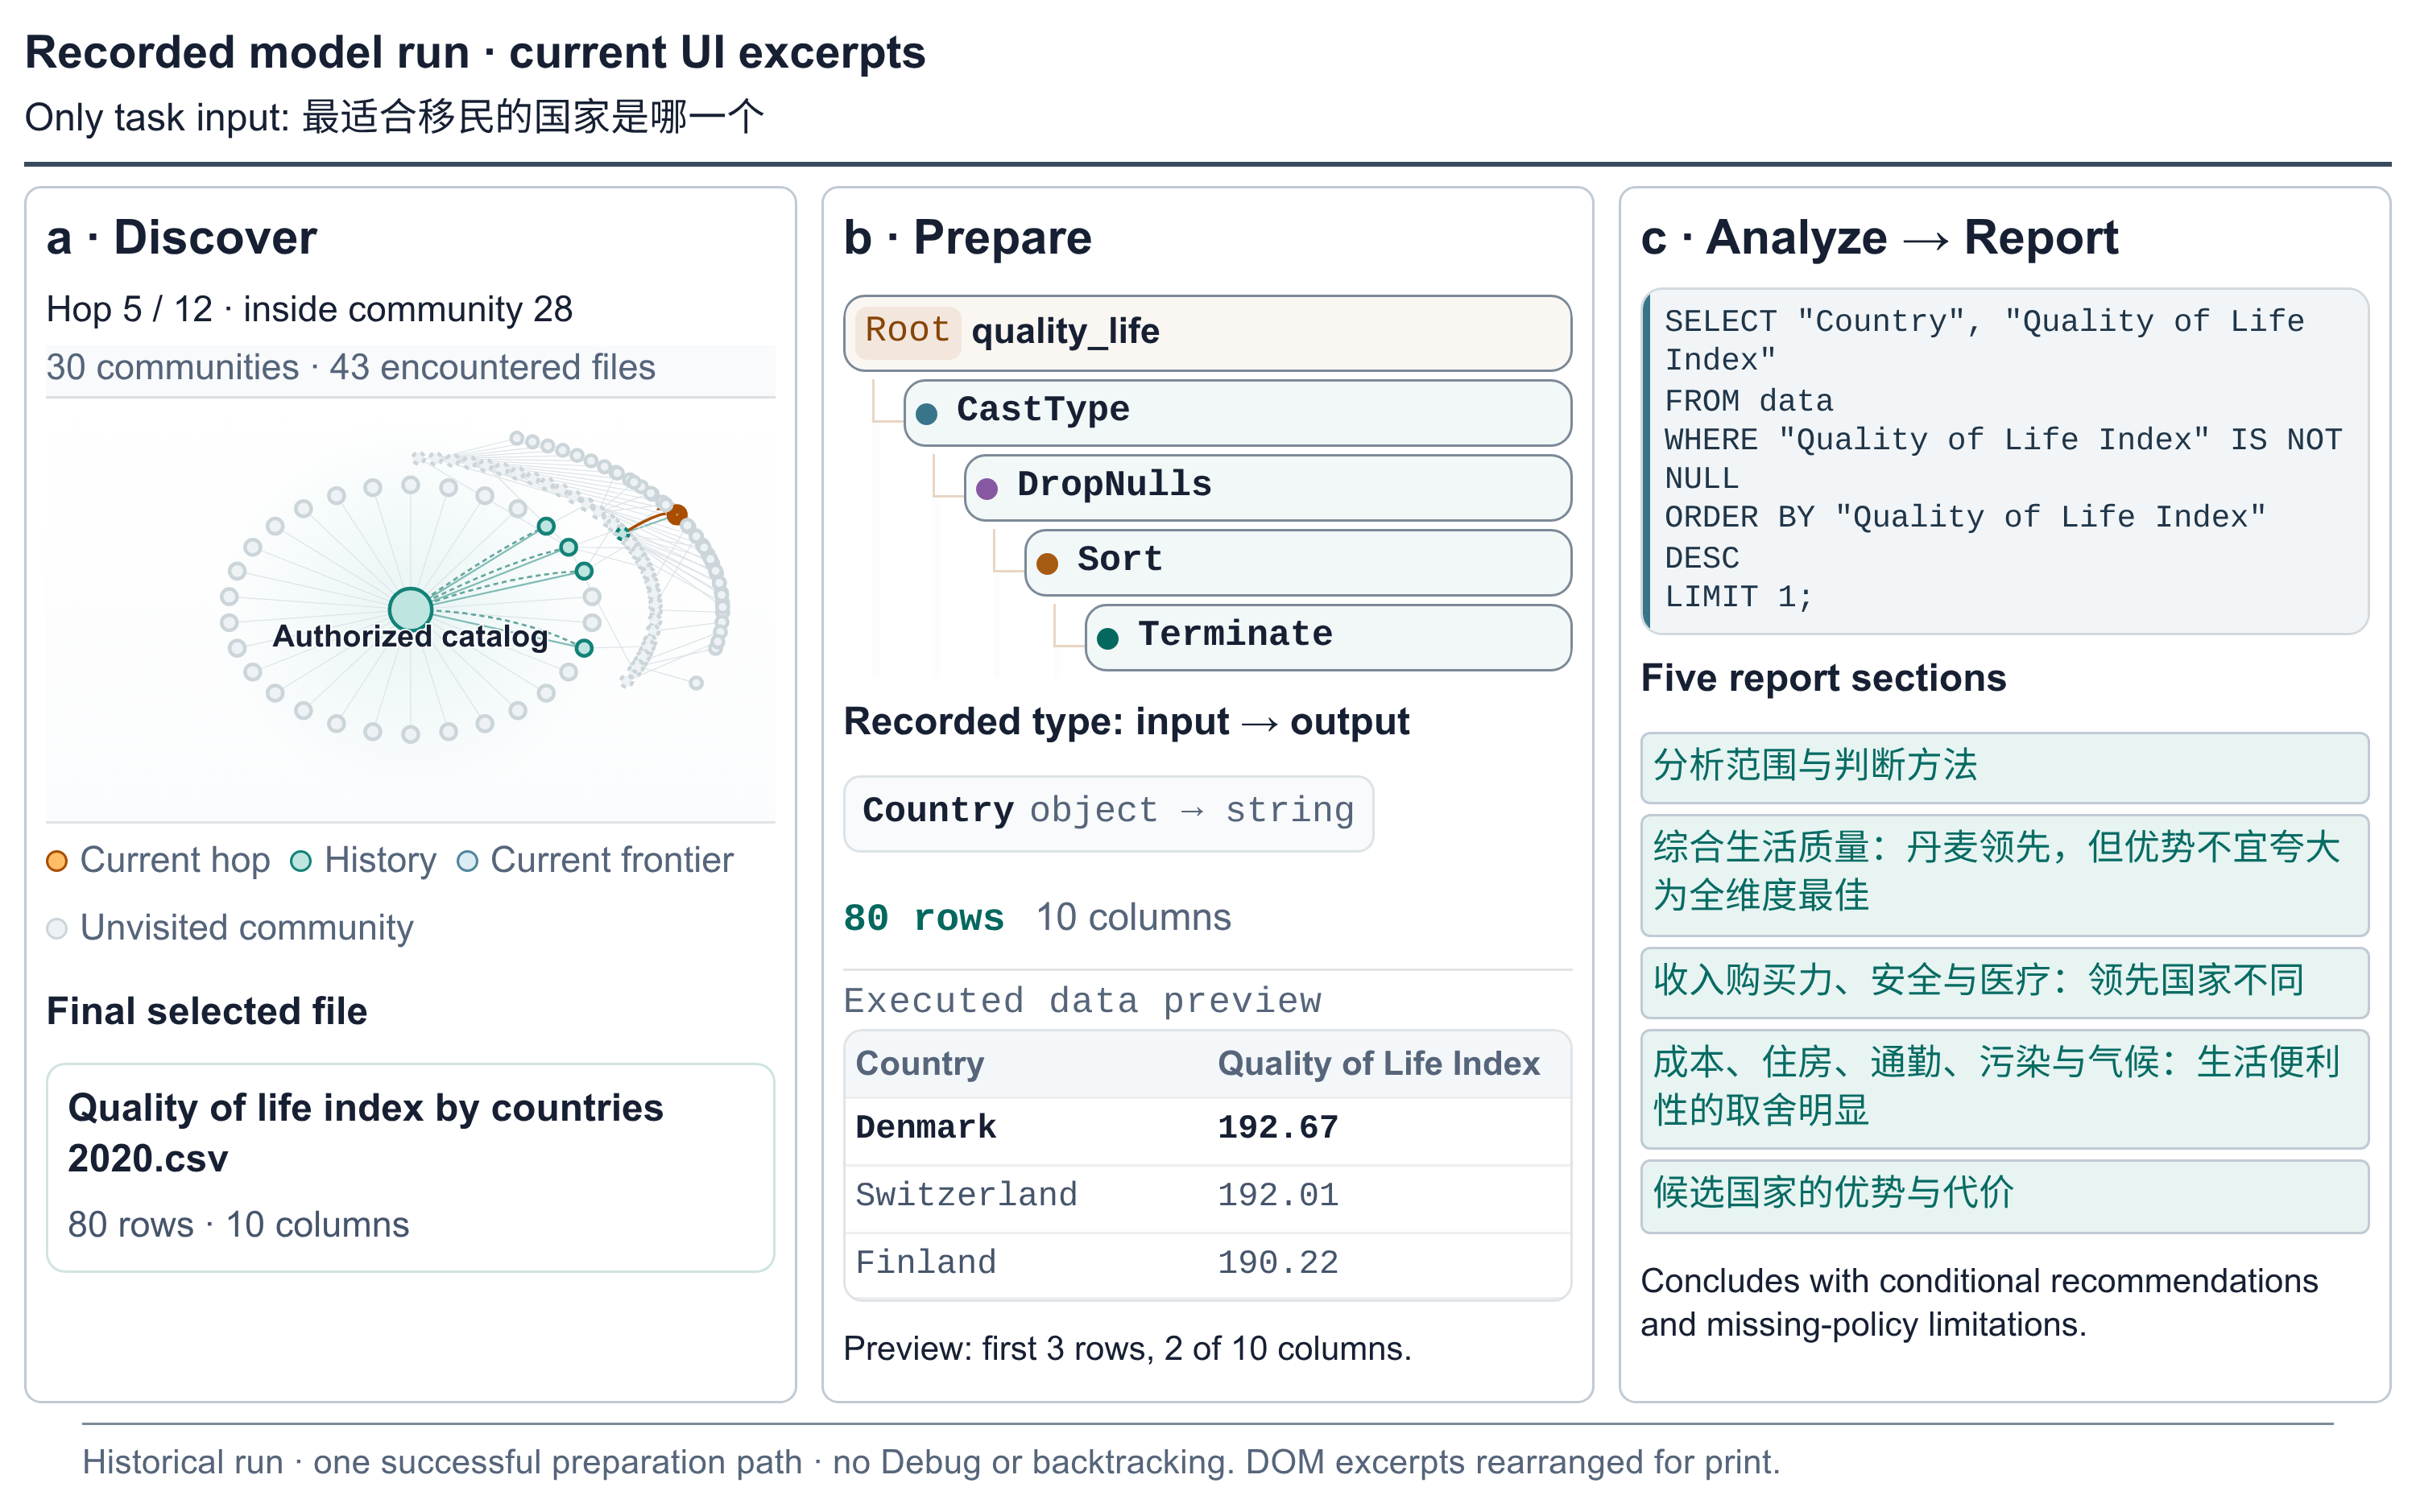
\includegraphics[width=0.995\textwidth]{figures/agentic-replay-v1/overview.png}
  \caption{Recorded model run in the current UI; excerpts rearranged for print.
  (a) Community exploration at hop 5 and the final file selected at hop 12.
  (b) The executed preparation path, recorded type difference, and table excerpt.
  (c) Executed SQL and five native-language report sections distinguishing overall
  quality, individual dimensions, and trade-offs. This run contains no backtracking or Debug.}
  \Description{Three panels replay a historical Chinese question about immigration.
  A community graph distinguishes the current hop from history. A four-operator
  preparation path leads to an 80-row table, of which three rows and two columns
  are shown. SQL and five report-section titles lead to conditional conclusions
  and explicit missing-policy limitations.}
  \label{fig:interface}
\end{figure*}

\subsection{Feasibility Evidence and Limitations}

We compare the same deterministic compiler, catalog, preparation, and analysis
operators under four controllers over all 15 \texttt{community\_43} questions.
Linear allows no repair.  Static retry allows two rounds but always reuses the
initial discovery terms; closed loop has the same budget but substitutes terms
from each typed violation.  Full profile reads every authorized source before
analysis and performs no repair.

\begin{table}[H]
  \caption{Controller outcomes on the complete 15-task community. ``Profiles''
  counts logical full-content profiles independently per task.}
  \label{tab:results}
  \small
  \begin{tabular}{lrrr}
    \toprule
    Controller & Correct terminal & Repair edges & Profiles \\
    \midrule
    Linear & 11/15 & 0 & 14 \\
    Static retry & 13/15 & 7 & 21 \\
    Closed loop & 15/15 & 4 & 18 \\
    Full profile & 15/15 & 0 & 150 \\
    \bottomrule
  \end{tabular}
\end{table}

Static retry recovers two of the four linear failures but exhausts its budget on
tasks 175 and 959, taking seven backward edges and 21 profiles.  In contrast,
violation-specific repair recovers all four with four edges and 18 profiles;
it exactly matches all 14
answerable oracles and correctly stops on the audited missing-source task.  Full
profile reaches the same terminal outcomes but logically exposes 1.356\,GB
versus 7.48\,MB.  Every mode first indexes paths and CSV headers, so these are
workload-exposure rather than physical-I/O or latency measurements.  Two
registered skewness tasks from \texttt{community\_52} also select the intended
source and match 2/2 answers.  After one warm-up per
scenario, 40 serial same-host requests through the production Nginx--FastAPI
path had median/P95/maximum latency of $21.5/57.9/58.4$\,ms.  This measurement
excludes startup, TLS, WAN delay, browser rendering, and model calls.

This remains a mechanism check: task families were registered after inspection,
each deterministic mode ran once, and static retry isolates repair-query
guidance only within that registry.  The second-community probe is not held out.
A 13-task community was selected while blinded, but its model-compiler run
has not occurred; that protocol does not cover the full agentic workflow.
Equal-model/budget baselines, repetitions, physical costs,
and narrative factuality evaluation remain.  Offline scenarios need neither
a GPU nor an external API.  The ECS profile has configuration checks but no
observed public deployment; authentication and isolated workers remain future
engineering work.

\balance
\section{Conclusion}

\systemname{} connects an analytical question to revisable source decisions,
materialized preparation, and report evidence.  Attendees inspect community
hops, candidate outputs, executed cells, and the backward repair edge without
choosing data themselves.  Controlled results establish mechanism feasibility;
model-based held-out evaluation and report factuality assessment remain
necessary for broader effectiveness claims.

\begingroup
\interlinepenalty=10000
\bibliographystyle{ACM-Reference-Format}
\bibliography{references}
\endgroup

\end{document}
\endinput
